\begin{figure}[h] 
\centering 
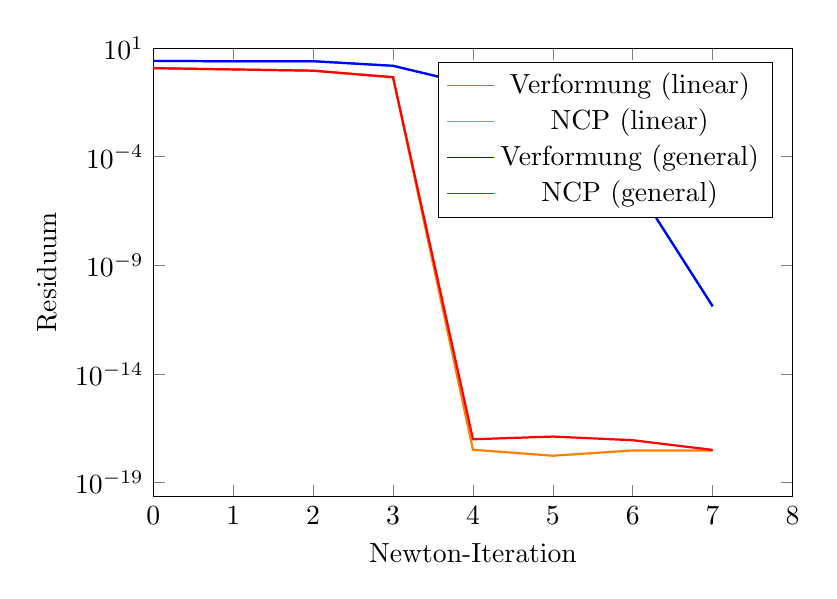
\begin{tikzpicture}[every plot/.append style={thick}] 
\begin{axis}[ 
label style={font=\normalsize}, 
xlabel={Newton-Iteration}, 
ylabel={Residuum}, 
xmin=0, xmax=8, 
ymode=log, 
ymin=0, ymax=10, 
width=0.8\textwidth, 
height=0.6\textwidth, 
legend pos=north east, 
legend style={cells={align=left}}, 
grid style=dashed, 
] 
\addplot[ 
color=cyan, 
] 
coordinates { 
(0, 2.60e+00)(1, 2.48e+00)(2, 2.51e+00)(3, 1.54e+00)(4, 2.03e-01)(5, 6.09e-03)(6, 7.52e-06)(7, 1.31e-11)}; 
\addlegendentry{Verformung (linear)} 
\addplot[ 
color=orange, 
] 
coordinates { 
(0, 1.20e+00)(1, 1.05e+00)(2, 9.18e-01)(3, 4.59e-01)(4, 3.26e-18)(5, 1.73e-18)(6, 3.02e-18)(7, 3.02e-18)}; 
\addlegendentry{NCP (linear)} 
\addplot[ 
color=blue, 
] 
coordinates { 
(0, 2.60e+00)(1, 2.48e+00)(2, 2.51e+00)(3, 1.54e+00)(4, 2.03e-01)(5, 6.09e-03)(6, 7.52e-06)(7, 1.31e-11)}; 
\addlegendentry{Verformung (general)} 
\addplot[ 
color=red, 
] 
coordinates { 
(0, 1.20e+00)(1, 1.05e+00)(2, 9.18e-01)(3, 4.59e-01)(4, 9.90e-18)(5, 1.32e-17)(6, 8.95e-18)(7, 3.20e-18)}; 
\addlegendentry{NCP (general)} 
\end{axis} 
\end{tikzpicture} 
\caption{Residuen des Stoffgesetzes 'St.Venant' mit Hinderniss 'Spitze' und 162 Freiheitsgraden für die Verschiebung.} 
\label{fiq:St.Venant_Spitze_level2} 
\end{figure} 
